\chapter{Introduction}
Nanophotonic devices are key building blocks in emerging technologies such as on-chip lasers, high-speed modulators, and quantum photonic platforms. 
These systems must operate reliably under real-world conditions: lasers must manage thermal and electrical effects, modulators must respond efficiently 
to electrical or thermal signals, and quantum devices must carefully mitigate (or utilize) mechanical and electromagnetic phenomena. In all these cases, device 
performance arises from the interaction of multiple physical domains, including electromagnetism, heat transfer, mechanics, and carrier dynamics.

Despite this inherently multiphysics nature, most current design approaches treat these effects in isolation or overlook them entirely. Designs are typically optimized 
for idealized optical performance, while non-optical effects are considered only a posteriori,
often resulting in suboptimal or unstable devices. This gap between idealized design models and real-world device behavior limits the scalability and robustness of current nanophotonic technologies.

One reason for this limitation is that conventional design methods rely on well-established, single-physics models (e.g., photonic crystals and waveguides), while the full multiphysics problem often remains conceptually and computationally challenging.
However, when thermal, mechanical, or electrical effects strongly influence the optical response, neglecting them in the design phase can compromise overall device performance.

This Ph.D. project aims to address these challenges by developing and applying multiphysics topology optimization methods for nanophotonic device design. These methods enable the simultaneous treatment of coupled physical effects, 
allowing for the automated discovery of device geometries that are not only optically efficient but also account for and utilize thermal, mechanical, and electrical effects. Beyond improving device reliability, this approach can reveal 
novel design principles and physical phenomena that emerge only when multiple physics are considered simultaneously.

\section{Multiphysics effects in nanophotonics}\label{intro:multi}

Multiphysics effects play a crucial role not only in advanced nanophotonic technologies but are also abundant in nature, where the interplay of optics with mechanics, thermodynamics, and chemistry creates dynamic and functional nano-optical systems.

\begin{figure}[b!]
    \centering
    \makebox[\textwidth][c]{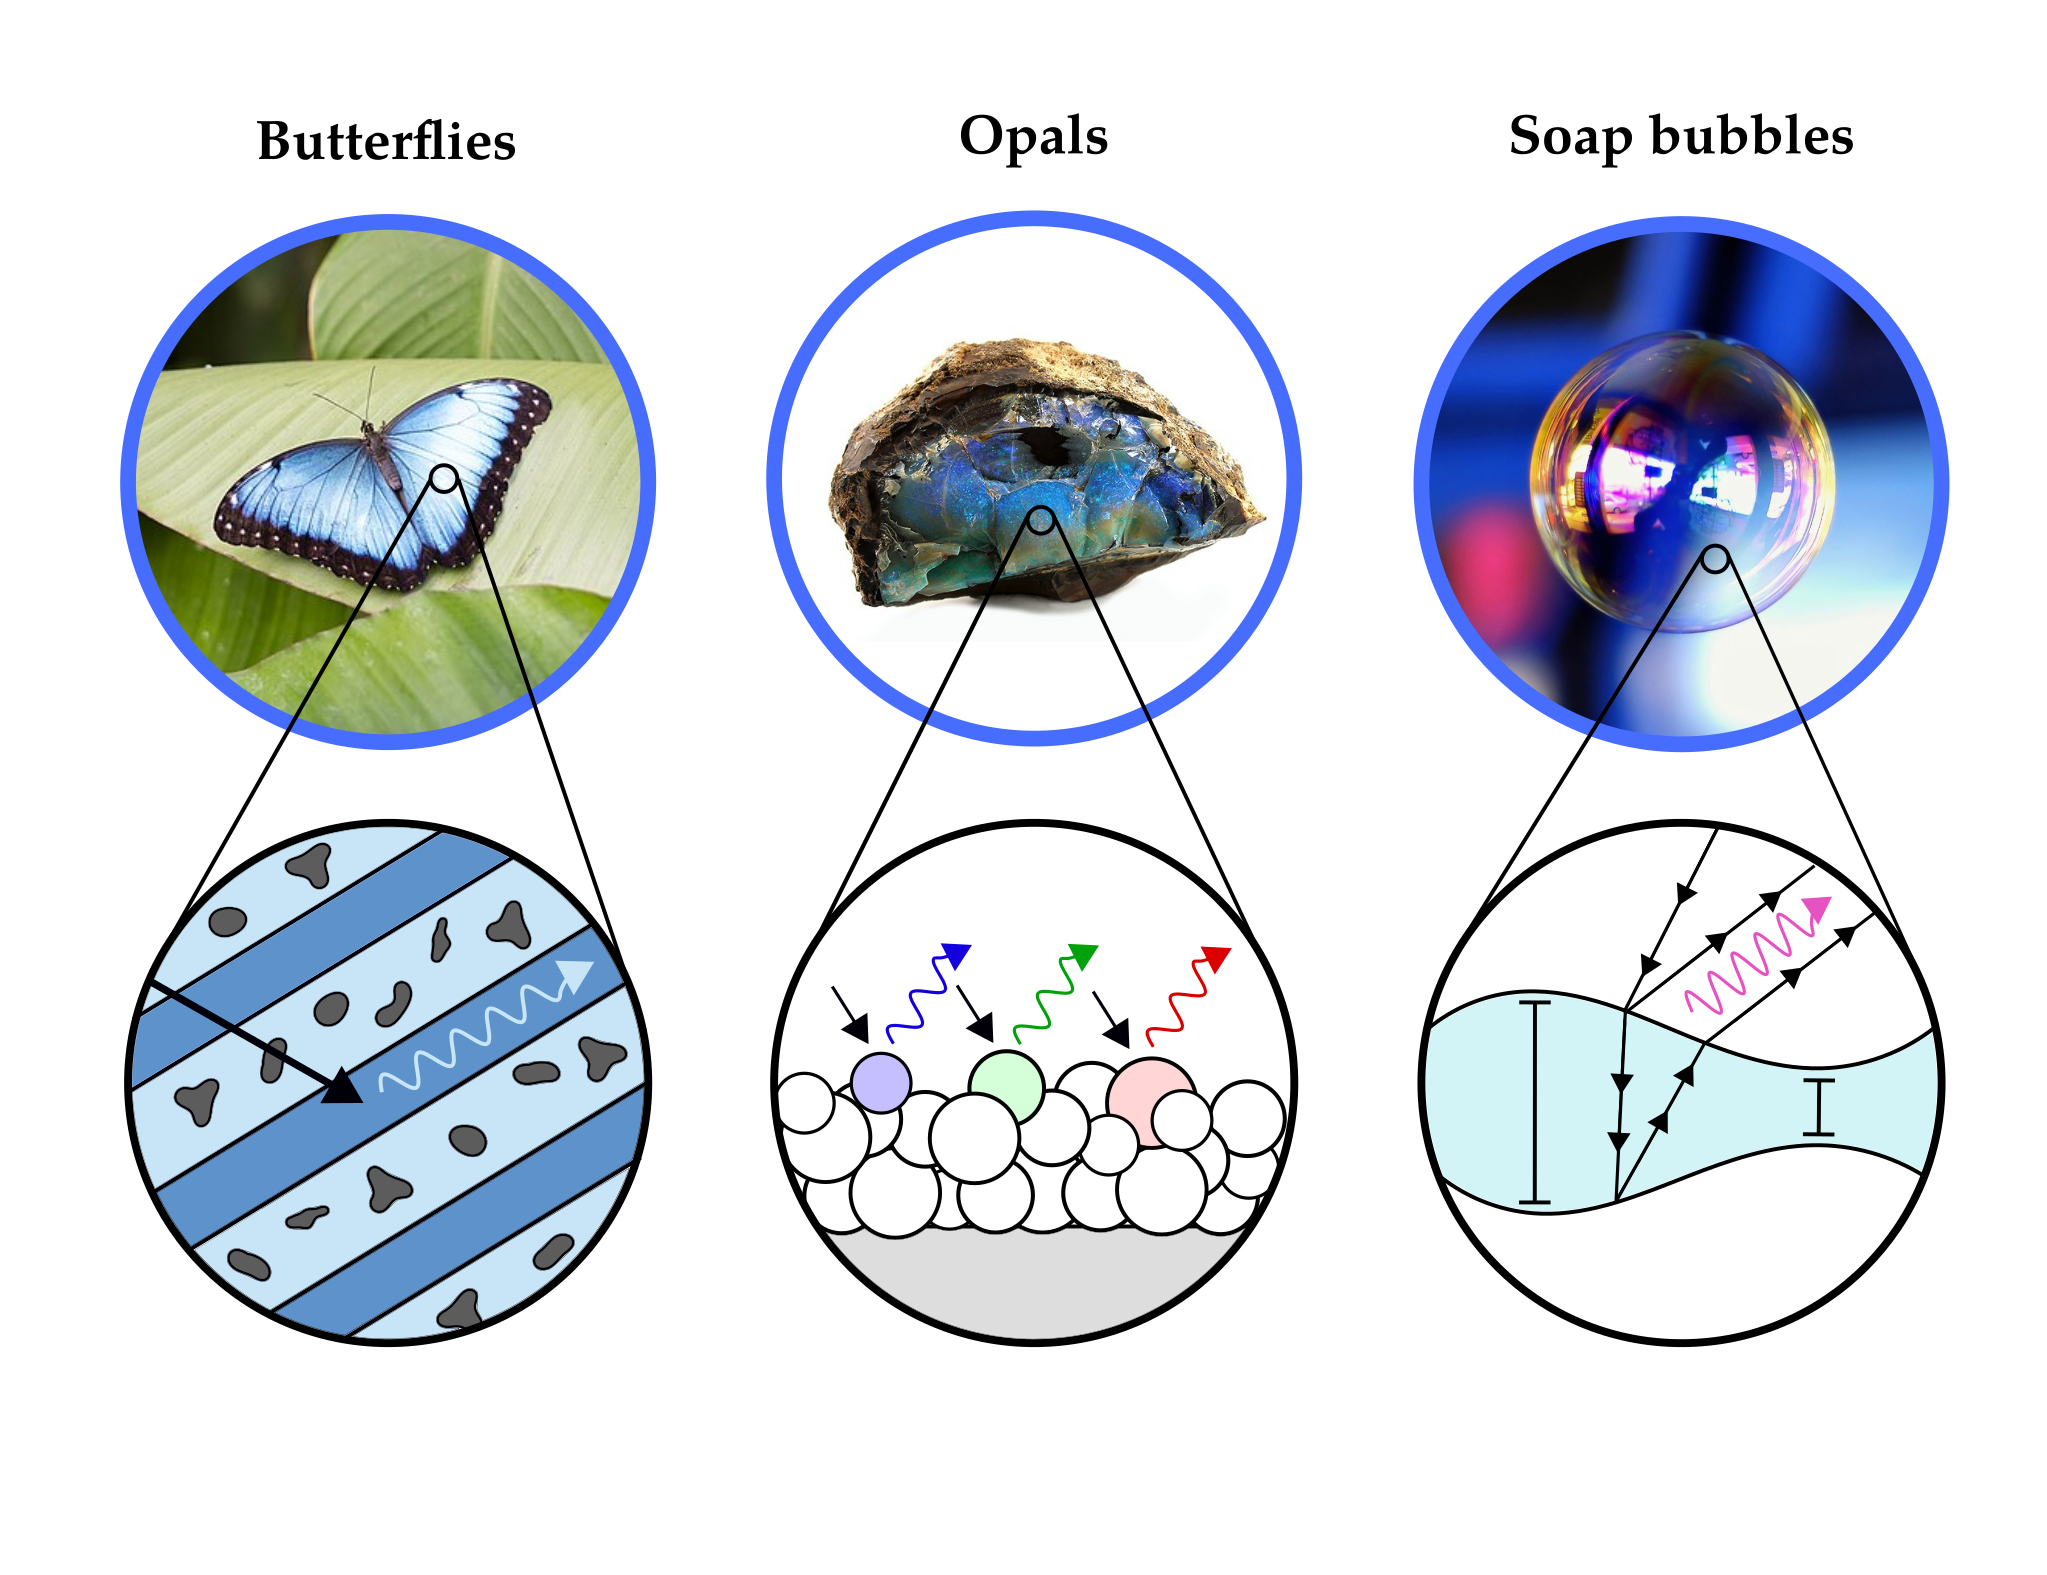
\includegraphics{figures/motivation_natural.png}}%%
    \caption{Macroscopic examples of nano-optical systems that exhibit multiphysics effects in nature. On the left, the vivid blue color of the \textit{Morpho peleides} butterfly (by Mira Meijer, Burgers' Zoo, \href{https://creativecommons.org/licenses/by-sa/4.0/}{CC BY-SA 4.0}) caused by its nanostructured wings. On the right, the iridescent patterns in soap bubbles (by Jeff Kubina, \href{https://creativecommons.org/licenses/by-sa/2.0/}{CC BY-SA 2.0}) caused by variations in its nanoscale film thickness. Photograph source: \href{https://commons.wikimedia.org/wiki/Main_Page}{Wikimedia commons}.}
    \label{fig:motivation_natural}
\end{figure}

As shown in \figref{fig:motivation_natural}, nature provides colourful examples of such multiphysics interactions. For instance, \textit{Morpho peleides} butterfly wings exhibit structural coloration caused by light interacting with nanoscale photonic structures in the wing scales~\cite{butterfly}. This coloration dynamically changes with mechanical deformation of the wings, variations in the angle of light incidence, and environmental factors such as humidity and temperature~\cite{morpho_temp}, which alter the physical properties of the nanostructures. 
Another striking example is the soap bubble, where iridiscent colors arise from thin-film interference effects within the nanoscale thickness of the soap film. The bubble's color shifts as the film thickness changes due to fluid flow, mechanical stresses, evaporation (linked to temperature changes), and chemical composition variations~\cite{bubble}, demonstrating strong coupling between fluid dynamics, thermal and chemical dynamics, and optics.

In engineered nanophotonics, multiphysics couplings are fundamental to various key applications. From photonic integrated circuits that tune light through  
thermo-optic~\cite{TOPS_1, TOPS_2, TOPS_3, program, PIC} and electro-optic~\cite{modu, modu1, modu2, pockels} effects, to nanolasers that balance optical gain, carrier dynamics, and heat dissipation~\cite{laser,laser_pic}, multiphysics couplings enable stable, efficient on-chip light manipulation. Equally, sensors  
push sensitivity limits by coupling electromagnetic fields with mechanical motion, thermal gradients, or chemical environments, to achieve unprecedented sensitivities \cite{therm_sensing,sensing, weakforce}.
Precise optomechanical manipulation, wheth\-er trapping nanoparticles~\cite{ashkin_acceleration_1970} or actuating tiny structures with light~\cite{ivanyi_optically_2024}, further illustrates how forces and electromagnetic fields work together at the nanoscale. Quantum photonic devices 
also leverage electrical, mechanical, and thermal effects to preserve quantum coherence, or achieve robust state manipulation~\cite{quant_eo, Andrews_2014, Xi_2025}. Bridging these advances, nano-opto-electro-mechanical systems (NOEMS)~\cite{NOEMS} uniquely integrate most of these  
domains, allowing electrical actuation, mechanical motion, and optical response to coexist in ultra-compact, reconfigurable platforms. 

% Wikimedia commons:
% 1. https://commons.wikimedia.org/wiki/File:Peleides_blue_morpho_(Morpho_peleides).jpg
% 2. https://commons.wikimedia.org/wiki/File:Opal-53714.jpg
% https://www.reddit.com/r/educationalgifs/comments/56sg9x/a_butterflys_wings_can_change_color_when_soaked/
% Bubble: https://commons.wikimedia.org/wiki/File:Bubble_brokenchopstick.jpg
%Sources:
%The GIF came from this video

%Ding, Y. Structural colors from Morpho peleides butterfly wing scales. J. Appl. Phys. 2009: 106, 074702

%Van Hooijdonk, E., et al. Detailed experimental analysis of the structural fluorescence in the butterfly Morpho sulkowskyi (Nymphalidae) J. Nanophoton. 2011: 5(1), 053525
\section{Topology optimization in nanophotonics}\label{intro:to}

As illustrated by the examples in the previous section, ingeniously engineered nanostructures and material properties play a crucial role in the
optical response of a system. Inspired by these natural structures, an overarching goal of nanophotonic
design is to optimize the geometry and material properties of the system to achieve a target
optical response.

\textbf{Topology optimization}~\cite{topopt_book} is a systematic inverse design method that effectively addresses this challenge. It finds the optimal distribution of material within a given design domain to maximize a target performance metric,
 known as the objective function or \textbf{figure of merit (FOM)}, while satisfying a set of constraints. This method
was pioneered in the field of structural mechanics by Bendsøe and Kikuchi~\cite{bendsoe_kikukchi}, 
and has since been extended to various fields, including fluids~\cite{topopt_fluid}, acoustics~\cite{topopt_acoustic}, 
electromagnetics~\cite{topopt_EM}, (nano)photonics~\cite{topopt_phot}, and multiphysics problems (\secref{sec:topopt_theory})~\cite{coupled_topopt}. In this thesis, we focus on the application of density-based~\cite{bendsoe_density, topopt_approaches} 
topology optimization in multiphysics nanophotonic problems~\cite{jensen_review}.

\textbf{Density-based topology optimization} describes the distribution of materials within a design space using a 
density\footnote{Note that this \emph{density} does not correspond to a physical material density, but rather represents a design variable used to describe the material distribution.} field or \textbf{design field} $\rho(\mathbf{r}) \in [0,1]$, where $\mathbf{r}$ is the position vector, $\rho = 0$ corresponds to one material, typically air or void, and $\rho = 1$ corresponds to a solid material.
 As illustrated 
in \autoref{fig:top_opt} for a nanophotonic system, the objective is to optimize the arrangement of these materials within 
the design domain to achieve a desired performance (e.g., maximizing transmission, reflection, absorption) when illuminated by a light source, such as a laser beam, an LED, or a focused light beam. 
The structure consists of passive regions, where the material remains fixed (e.g., void in \figref{fig:top_opt}), and design regions, where the material distribution 
is optimized. The optimization process iteratively updates the design field until the FOM is maximized or minimized, and the targeted optical response is achieved.

\begin{figure}[tb]
    \centering
    \makebox[\textwidth][c]{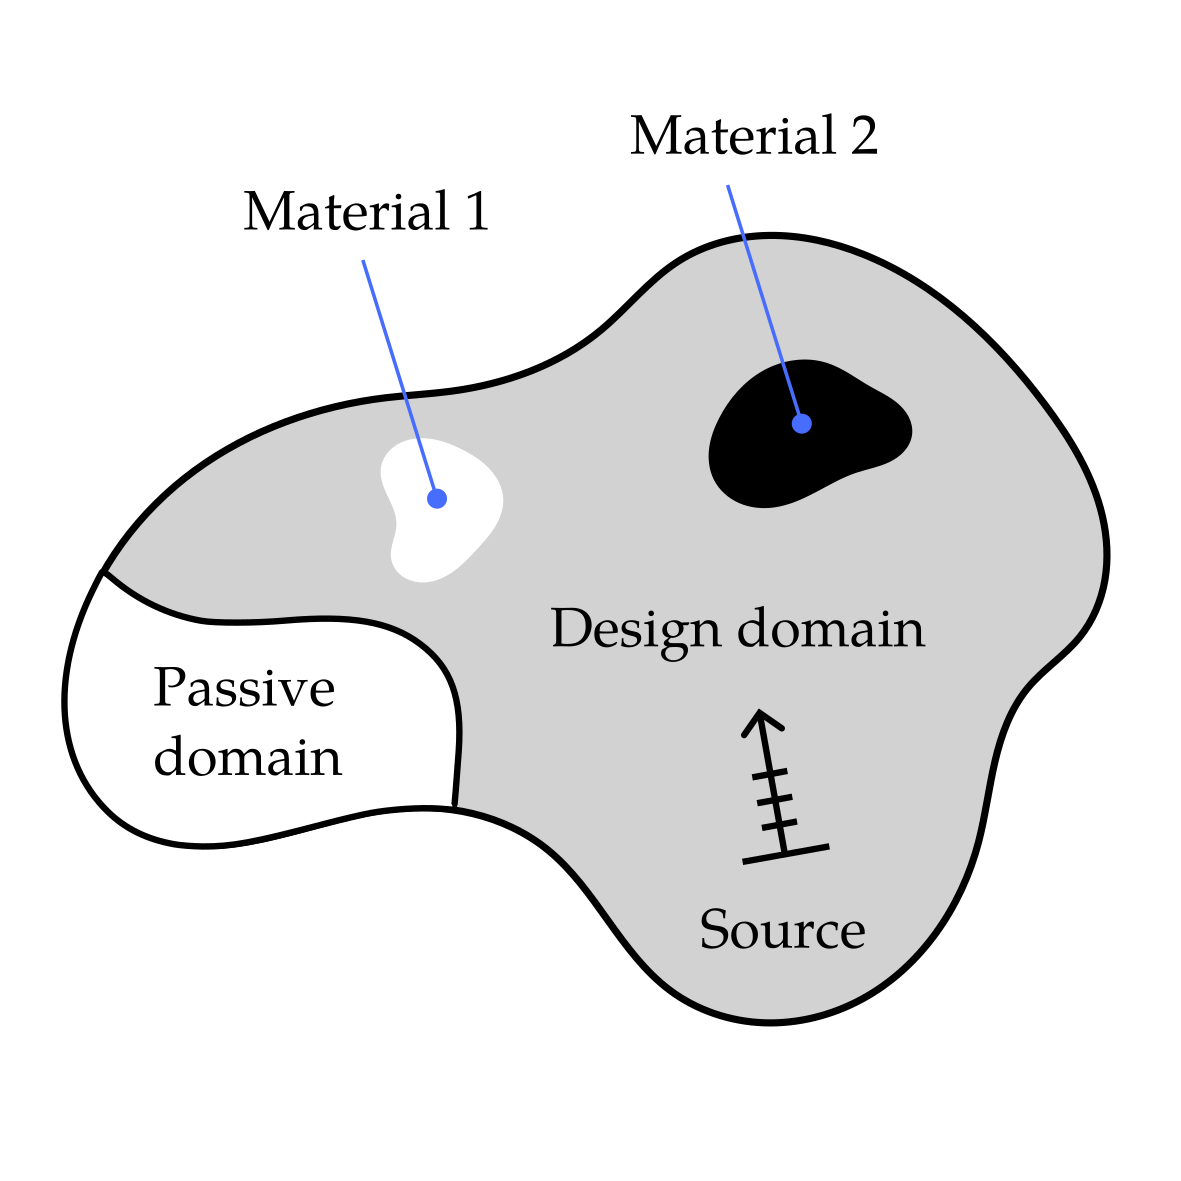
\includegraphics{figures/top_opt.png}}%%
    \caption{Topology optimization of a nanophotonic system, that is excited by an optical source. The simulation domain comprises a passive domain (white) where the material is fixed, and a design domain (grey), where the material distribution is optimized for two different materials.}
        \label{fig:top_opt}
\end{figure}

For further details on inverse design by density-based topology optimization in photonics and nano-optics, we refer the reader to
the review papers by Jensen and Sigmund~\cite{jensen_review} and the more recent one by Molesky et al.~\cite{Molesky_2018}. 
For an introduction focusing on practical implementation, we refer the reader to the tutorial papers by Christiansen and Sigmund~\cite{tutorial_matlab, tutorial_COMSOL}.

\section{Structure of the thesis}

This thesis combines the concepts presented in \secref{intro:multi} and \secref{intro:to} by addressing multiphysics topology optimization problems in nanophotonics. The following chapters focus on reviewing
 the theoretical framework, presenting the contributions of this thesis in the context of state-of-the-art research,
  and concluding the thesis with a summary and a discussion of future research directions.

  \textbf{Chapter 2} introduces the theoretical framework used throughout the thesis, including the mathematical formalism
  to describe the propagation of light in nanophotonic systems (\secref{sec:nanophotonics}), the basics for the numerical implementation of 
  finite element-based simulation tools (\secref{sec:fem}), and the theory behind inverse design by topology optimization in multiphysics systems (\secref{sec:topopt_theory}).
  
  \textbf{Chapter 3} covers thermo-optically coupled topology optimization problems, with 
  special emphasis on the topology optimization of thermo-optical phase-shifters (\secref{sec:TOPS})~\cite{ownpub0}.

  
  \textbf{Chapter 4} addresses optomechanically coupled topology optimization problems, highlighting the topology optimization of optical force-based particle systems (\secref{sec:engi})~\cite{ownpub2}, integrated optical trapping cavities (\secref{sec:dip})~\cite{ownpub1, ownpub3}, and strongly coupled optomechanical
  problems, such as optomechanical membrane devices (\secref{sec:mech_strongly_coupled})~\cite{ownpub5}.
  
  \textbf{Chapter 5} explores electro-optically coupled topology optimization problems, with special focus on the topology optimization of 
  nanolaser devices (\secref{sec:laser})~\cite{ownpub4}.
  
  \textbf{Chapter 6} concludes the thesis by summarizing the main results and outlining potential directions for future research in the field.

This thesis comprises a collection of papers~\cite{ownpub0, ownpub1, ownpub2, ownpub3} and manuscripts~\cite{ownpub4, ownpub5} that
are included in Sec.~\hyperref[sec:publications]{Publications}.